%!TEX ROOT=../ctutest.tex

\chapter{State of the Art}
%--- FIG: UTF forms

This chapter will first describe the originally popular models for NLP such as BERT and the recent paradigm shift from \textit{pre-train+fine-tune} transfer learning framework popular since the original~\cite{devlin2019bert} paper to the currently booming LLMs which often outperform the smaller models even without the fine-tuning step~\cite{gpt4,llama,vicuna}. We will then take a look at the performance optimization methods that enable training multi-billion parameter pre-trained models on a set of task-specific data on a single GPU and their potential for our research. 

\label{chap:sota}
\section{Pretrain + Finetune}
\label{sec:pretrain}
For the last decade, the \textit{pretrain-finetune} paradigm has been a cornerstone in the field of Natural Language Processing (NLP) and has significantly shaped the development of modern NLP models. Its history in NLP can be traced back to the advent of neural networks and deep learning in the early 2010s. Initially, researchers pre-trained word embeddings using methods like Word2Vec~\cite{mikolov} and GloVe~\cite{pennington-etal-2014-glove} which captured semantic relationships among words. 

\subsection{BERT and derivatives}
The \textit{pretrain-finetune} paradigm truly rose to fame with the introduction of transformer-based models, particularly the revolutionary BERT (Bidirectional Encoder Representations from Transformers) in 2018. BERT~\cite{bert} demonstrated the power of pretraining large-scale language models on massive text corpora using an easy-to-automate general task such as \textit{Masked Language Modeling}, or \textit{Next Sentence Prediction}, followed by fine-tuning on specific downstream tasks using smaller, harder to obtain data. This approach achieved state-of-the-art results across various NLP benchmarks. Subsequently, numerous variations of pre-trained models like GPT (Generative Pre-trained Transformer) and RoBERTa emerged, each refining the pretrain-finetune paradigm to improve language understanding, generation, and transfer learning capabilities. 

Importantly, BERT's success inspired a number of publications in training similar transformer models, varying in the definition of the general pre-training task, model size, architecture training corpus

\begin{itemize}
    \item In Czech language, monolingual models CZERT~\cite{czert}, FERNET~\cite{fernet}, RobeCzech~\cite{straka2021robeczech}, and small-e-czech~\cite{kocian2021siamese} are available for further finetuning
    \item In Polish, HerBERT~\cite{mroczkowski-etal-2021-herbert} achieved state of the art in multiple tasks in 2021
    \item In Slovak, SlovakBERT~\cite{pikuliak2021slovakbert} was released by KInIT and Gerulata
    \item A multitude of multilingual models, such as \MBERT or \XLM~\cite{xlm-roberta} were pretrained on data in all three of these languages (and many others), proving that the large transformers can capture a notion of semantics and relations between pieces of text even \textit{without} the convenient constriction of a single language 
\end{itemize}

\section{Few-shot and Zero-shot learning}
\label{sec:llms}
The ever-growing (sometimes, billions of parameters) transformer models have not only demonstrated superior performance on benchmark datasets but have also shown remarkable zero-shot and few-shot learning abilities, where they can perform tasks with minimal or no task-specific training data~\cite{gpt3}.

Few-shot learning refers to the capability of a model to perform a task when provided with only a limited amount of labeled examples. Zero-shot learning takes this concept a step further by enabling models to tackle tasks they have never seen during training. The integration of these learning paradigms into large language models like GPT-3 and subsequent iterations has spread the NLP hype even further. By utilizing a prompt or a few examples, these models can quickly adapt to new tasks, making them highly versatile, adaptable and usable to the general public.
\subsection{GPT-3.5 and GPT-4}
\label{sec:gpt}
Obscure, paid~\cite{gpt3,gpt4}

\subsection{LLaMA-2 and derivatives}
\label{sec:llama}
Open-source, freely usable.
Often poor czech coverage 
Quantizace, 4b, 8b, zlomek parametrů\cite{openassistant}

\subsection{LoRA and other optimization}
To be able to fine-tune multi-billion-parameter models such as \textsf{LLaMA-2}~\cite{llama2} on a single TPU, multiple adjustments must be made to reduce the computational complexity.~\cite{peft}
\cite{lora}

\section{Fact checking approaches}
\subsection{FEVER and followups}
Yields interesting benchmark with statistically quantifiable model succes, oversimplificates the problem, as it uses Wikipedia for a trusted knowledge base and only reasons based on a data from a fixed period of time, focusing on \"{atomic} claims that do not match the complexity of real-world factoids.
\subsection{Open-domain fact-checking}
This paper with bing for example uses the whole internet, but is that really what we want? Like, every lie can be backed with an internet -- at the end of the day you do need to draw the line of what to trust somewhere, which directly conflicts this design.


\begin{figure}
    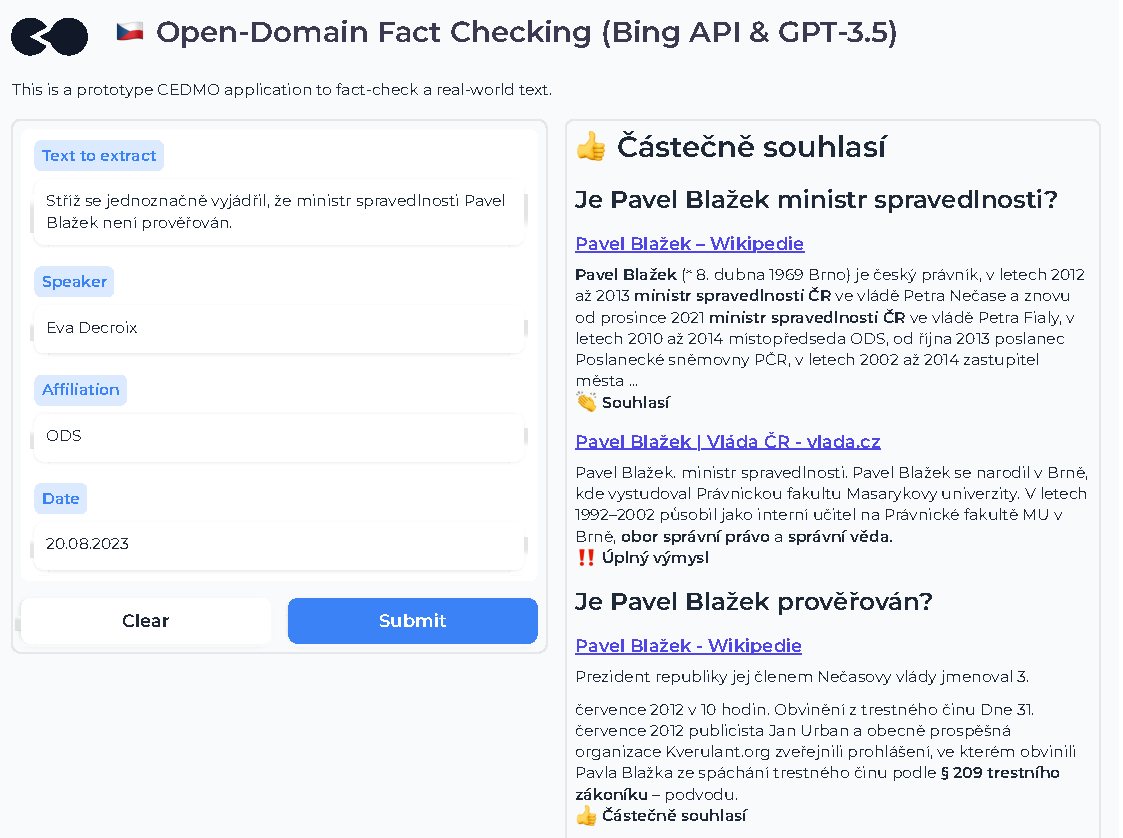
\includegraphics[width=14cm]{fig/bing.pdf}
    \caption{Proof-of-concept Czech fact-checking based on live-internet search (Bing API) and LLM prompting, based on the proposals of~\cite{bing} in Czech, using a real-world claim that was fact-checked by \href{https://demagog.cz/vyrok/22849}{\url{demagog.cz}} in June 2023}
    \label{fig:bing}
\end{figure}


\section{Claim generation}
\begin{itemize}
    \item Approches such as QACG exploit Question Answering
    \item The task of extreme summarization (XSum) focuses on summarizing a long body of text into a single sentence, focusing on its most relevant aspects and facts
    \item CLEF-CheckThat postulates the task of classifying \textit{Checkworthiness} of different parts of a long texts, such as a political debate
\end{itemize}

\section{NLP Generative task benchmarking}
\subsection{BERTScore}
\subsection{AlignScore}